\documentclass[12pt]{article}
\usepackage{multirow}
\usepackage{graphicx}
\usepackage{wrapfig}
\usepackage[T2A]{fontenc}			% кодировка
\usepackage[utf8]{inputenc}			% кодировка исходного текста
\usepackage[english,russian]{babel}	% локализация и переносы
\usepackage{amsmath,amsfonts,amssymb,amsthm,mathtools} 
\usepackage{hyperref}
\usepackage[rgb]{xcolor}
\usepackage{wasysym}
\usepackage{fancyhdr}
\pagestyle{fancy}
\usepackage[left=3cm,right=3cm, top=3cm, bottom=3cm, bindingoffset=0cm]{geometry}

\begin{document}
\begin{titlepage}
\begin{center}
\huge{Лабораторная работа № \textbf{4.3.3}}\\[1cm]\LARGE {Исследование разрешающей способности микроскопа методом Аббе\\[7 cm]}
\end{center}

\begin{flushright}
\Large{Карманов Алексей\\752 группа}\\[9 cm]
\end{flushright}
\begin{center}
г.Долгопрудный\\
20.02.2019
\end{center}
\end{titlepage}
\fancyhead[L]
\indent \textbf{Цель работы:}Определение дифракционного предела разрешения
объектива микроскопа методом Аббе.\\[0.75 cm]
\indent \textbf{В работе используются:} лазер, кассета с набором сеток разного периода, линзы, щель с микрометрическим винтом, оптический стол c набором рейтеров и крепёжных винтов, экран, линейка\\
\section{Теоретическая справка}
Разрешающей способностью оптического прибора называют минимальное расстояние $l_{min}$ между двумя точками в пространстве предметов, которое прибор может разрешить. При визуальном наблюдении изображения в качестве критерия разрешения применяют так называемый критерий Рэлея. \par
Для иммерсионного микроскопа (объект находится в иммерсионной среде — жидкости с показателем преломления n) разрешающая способность объектива при некогерентном освещении
\begin{equation}
    l_{min} = \frac{0.61 \lambda}{n \sin A},
\end{equation}

где A — апертурный угол объектива микроскопа. \par
Рассмотрим теперь когерентно освещённый объект, наблюдаемый в микроскоп. Схема образования изображения в объективе микроскопа
представлена на рис. 1.
    \begin{figure}[h]
    \centering
    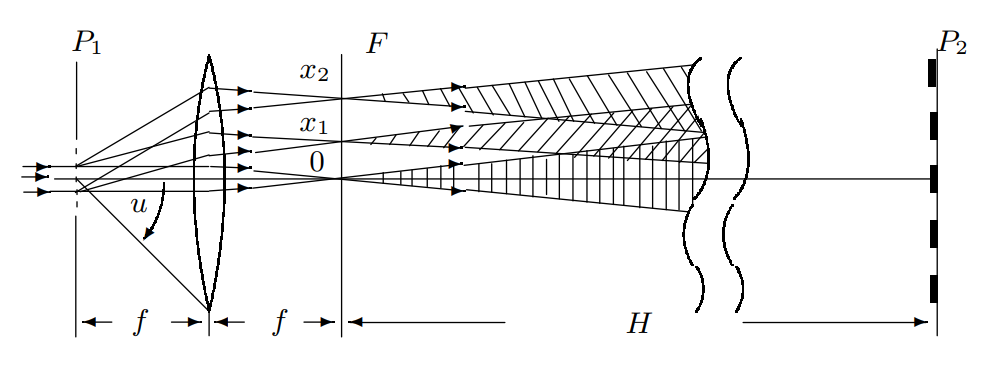
\includegraphics[width=15cm]{fig2.PNG}
    \caption{Образование изображения в объективе микроскопа. $P_1$ — плоскость предмета, $F$ — задняя фокальная плоскость объектива, $P_2$ — плоскость,
сопряжённая с предметной плоскостью. В плоскости $P_2$ световые пучки
сильно перекрываются}
    \label{fig:vac}
\end{figure}

минимальное разрешаемое объективом расстояние
определяется условием

\begin{equation}
    l_{min} = \frac{\lambda}{\sin A} \approx \frac{\lambda}{D/2f},
\end{equation}

где D — диаметр диафрагмы. При этом диафрагма, расположенная
симметрично, пропускает нулевой и $\pm1$ дифракционные максимумы.


\section{Экспериментальная установка}

Схема модели проекционного микроскопа приведена на рис. 2. Предметом служат сетки, расположенные
в кассете. Смена сеток осуществляется поворотом внешнего кольца кассеты.

    \begin{figure}[h]
    \centering
    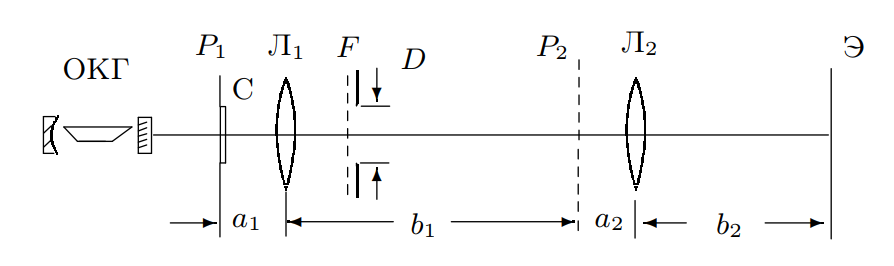
\includegraphics[width=15cm]{fig1.PNG}
    \caption{Схема экспериментальной установки — модель проекционного
микроскопа}
    \label{fig:vac}
\end{figure}

\section{Определение периода решёток по их пространственному спектру}
\begin{enumerate}
    \item Для определения периода решёток измерим расстояния между максимумами разных порядков на экране. Расстояние от сетки до экрана $D = 120$ см. Период решётки рассчитывается по формуле 
    \begin{equation}
        d = \frac{\lambda D}{d_{mes}}
    \end{equation}
    Результаты измерений занесём в таблицу 1.
    
        \begin{table}[h]
    \centering
    \begin{center}
    \caption{Периоды решёток, метод пространственного спектра}
    \end{center}
    \vspace{0.1cm}
    \label{tab:my_label}
    \begin{tabular}{ |p{3 cm}||p{1cm}|p{1cm}|p{1cm}|p{1cm}|p{1cm}|}
 \hline
Номер решётки & 1 & 2 & 3 & 4 & 5\\
 \hline
 $d_{mes}$, мм & 32.8 & 21.9 & 11.3 & 5.4 & 4.1 \\
 \hline
 $d$, мкм & 19.4 & 29.1 & 56.7 & 117.2 & 155.2\\

 \hline
 
\end{tabular}
\end{table}
\end{enumerate}

\section{Определение периода решёток по изображению, увеличенному
с помощью модели микроскопа}
\begin{enumerate}
    \item Соберём модель проекционного микроскопа (рис. 2), центрируем систему. Увеличение полученной системы вычисляется по формуле
    \begin{equation}
        \gamma = \frac{b_1 b_2}{a_1 a_2},
    \end{equation}
    (расстояния $a_1$, $a_2$, $b_1$, $b_2$ см на рис. 2)
    \item На экране измерим расстояния между максимумами разных порядков. Результаты измерений занесём в таблицу 2.
    
        \begin{table}[h]
    \centering
    \begin{center}
    \caption{Периоды решёток, по изображению с микроскопа}
    \end{center}
    \vspace{0.1cm}
    \label{tab:my_label}
    \begin{tabular}{ |p{3 cm}||p{1cm}|p{1cm}|}
 \hline
Номер решётки & 4 & 5\\
 \hline
 $d_{mes}$, мм & 9.0 & 11.8 \\
 \hline
 $d$, мкм & 108.9 & 170.2 \\

 \hline
 
\end{tabular}
\end{table}

\end{enumerate}

\section{Определение периодов решёток по оценке разрешающей способности микроскопа}
\begin{enumerate}
    \item Поместим щелевую диафрагму с микрометрическим винтом в фокальную плоскость $F$ линзы Л1. Определите для каждой решётки минимальный размер диафрагмы $D$, при котором на экране ещё видно изображение сетки (при меньших размерах щели изображение выглядит
как одномерная решётка). Результаты измерений занесём в таблицу 3.

        \begin{table}[h]
    \centering
    \begin{center}
    \caption{Периоды решёток, по измерению диафрагмы}
    \end{center}
    \vspace{0.1cm}
    \label{tab:my_label}
    \begin{tabular}{ |p{3 cm}||p{1cm}|p{1cm}|p{1cm}|}
 \hline
Номер решётки &  3 & 4 & 5\\
 \hline
 $D$, мм  & 1.7 & 0.8 & 0.6 \\
 \hline
 $d$, мкм  & 55.5 & 120.7 & 161.3 \\

 \hline
 
\end{tabular}
\end{table}

    \begin{figure}[h]
    \centering
    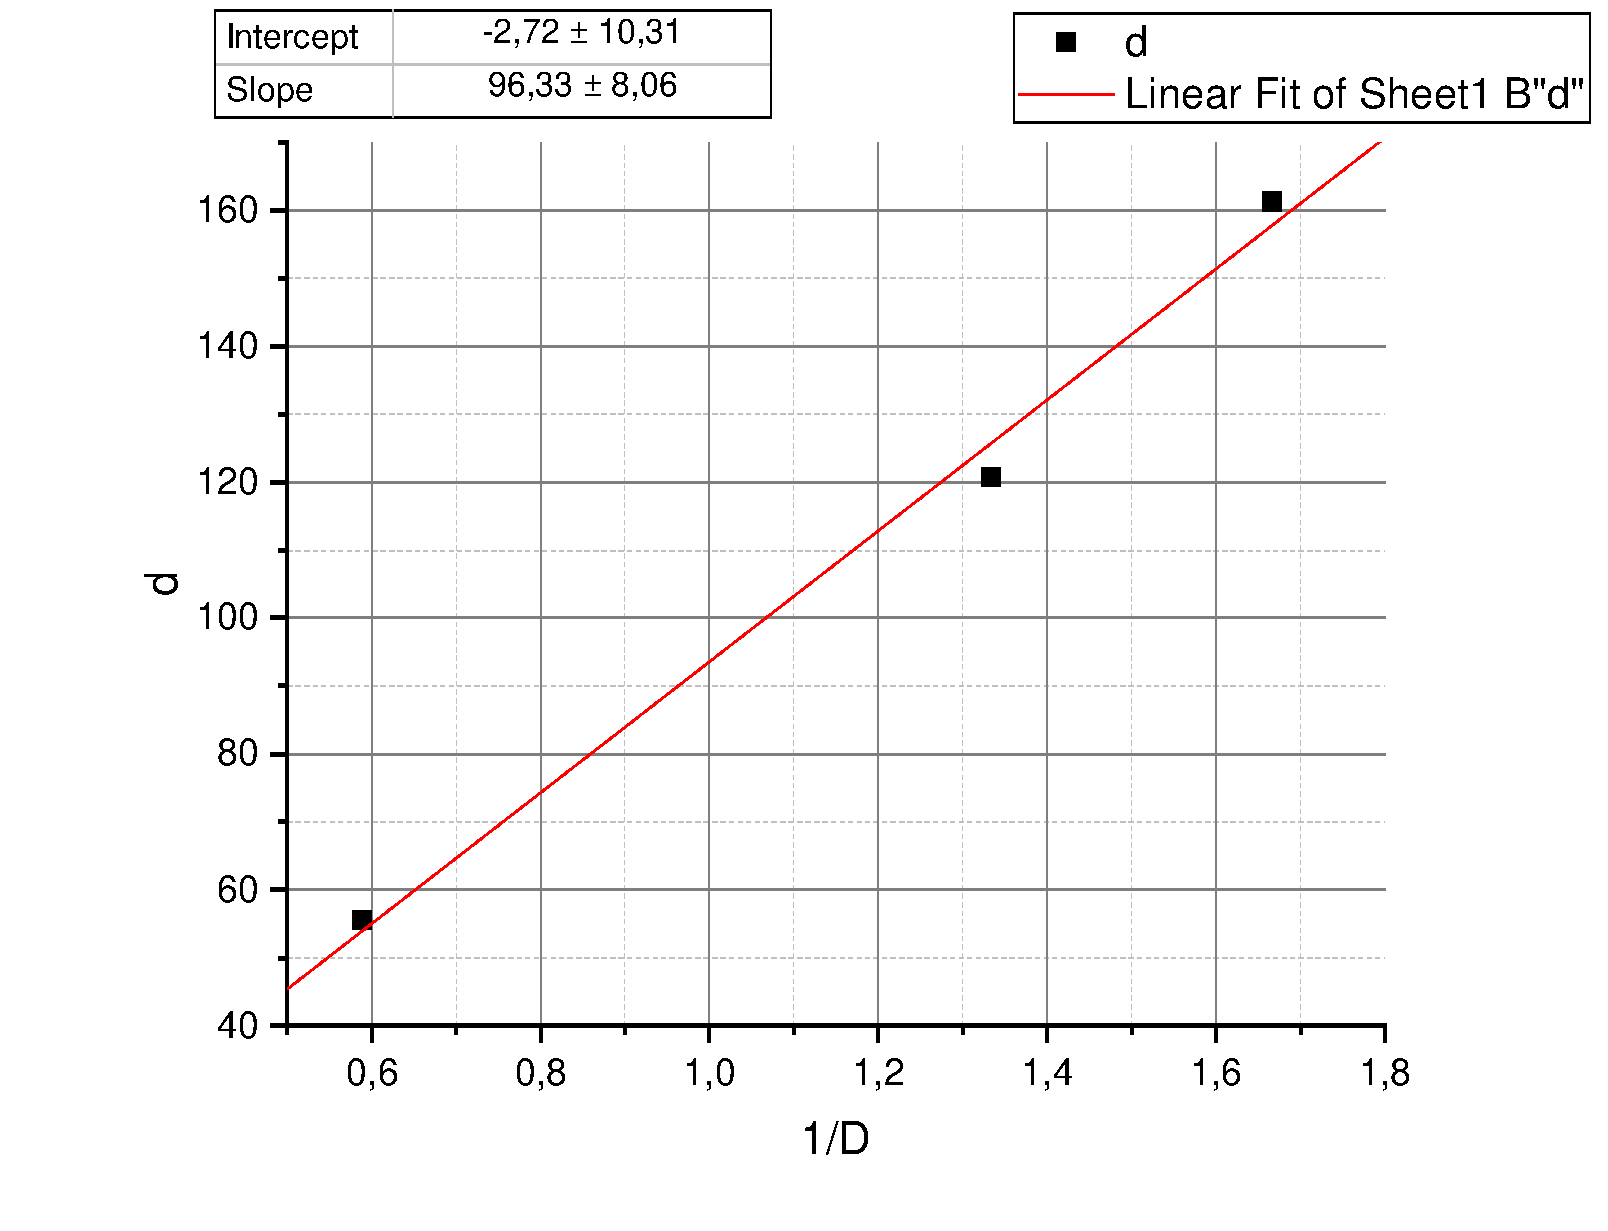
\includegraphics[width=13cm]{fig3.pdf}
    \caption{Зависимость d = f(1/D)}
    \label{fig:vac}
\end{figure}

\item Для проверки теории Аббе построим график зависимости d = f(1/D), взяв периоды сеток, определённые по спектру. Определим угловой коэффициент, он равен 130. По формуле $d \ge \frac{\lambda}{D/2f}$, тогда при наших условиях теоретический угловой коэффициент равен 154. Теория Аббе верна в пределах используемой точности.

\end{enumerate}

\section{Пространственная фильтрация и мультиплицирование}

Поворачивая щель относительно оси, добьёмся того, чтобы щель занимала наклонное положение под $45^\circ$. Тогда будет осуществляться пространственная фильтрация, то есть выделение из спектра максимумов $m_x = m_y$ (диагональных максимумов). Тогда на экране возникнет изображение решётки, которой нет на самом деле. Полосы располагаются под углом $45^\circ$, что видно на рисунке \ref{filtr}. Период новой решетки равен 0,852 мм, что в $\sqrt{2}$ раз больше периода изображения решётки, определённого стандартным методом (по увеличенному изображению решётки). Это объясняется тем фактом, что расстояние между выделенными максимумами, то есть между вторичными источниками волн, составляет $d\sqrt{2}$. Также наблюдали мультиплицирование, то есть рассечение фурье-образа щели сеткой. Такой эффект создаётся, если в нашей установке поменять местами сетку и щель.

\begin{figure}[h]
    \centering
    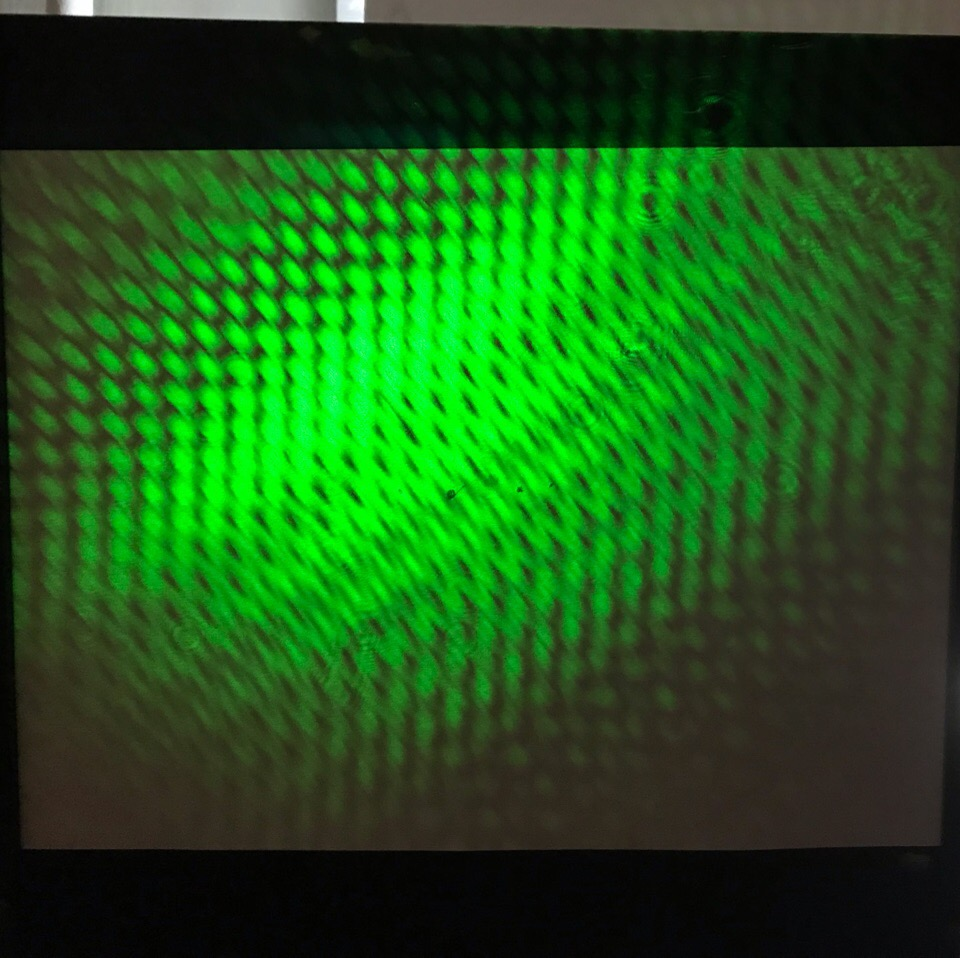
\includegraphics[width= 0.6\textwidth]{5.jpg}
    \caption{Пространственная фильтрация}
    \label{filtr}
\end{figure}


\begin{figure}[h]
    \centering
    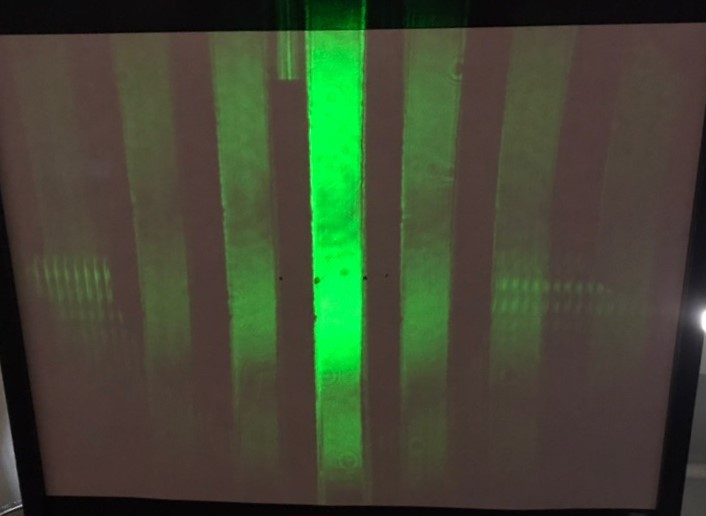
\includegraphics[width=0.6\textwidth]{6.jpg}
    \caption{Пространственное мультиплицирование}
    \label{filtr}
\end{figure}

\end{document}